\subsubsection{Prospetto Orario}
Di seguito è riportata la suddivisione oraria dei ruoli nel periodo di Pianificazione di dettaglio e codifica.




\begin{table}[H]	
	\begin{center}
	    \begin{tabular}{cccccccc}
			\rowcolor{greySWEight}
			\textcolor{white}{\textbf{Nome}} & \textcolor{white}{\textbf{Re}} & \textcolor{white}{\textbf{Am}} & \textcolor{white}{\textbf{An}} & \textcolor{white}{\textbf{Pj}} & \textcolor{white}{\textbf{Pr}} & \textcolor{white}{\textbf{Ve}} & \textcolor{white}{\textbf{Totale}}
			\\ 
			Bacco Alberto & & & 10 & 22 & & 20 & 52 \\
			Caccaro Sebastiano & & 5 & & & 32 & 15 & 52 \\
			Ciagola Damien & 5 & & & 27 & & 20 & 52 \\
			Corti Francesco & 5 & 5 & & & 22 & 20 & 52 \\
			Isachi Gheorghe & & & & 22 & 20 & 10 & 52 \\
			Legrottaglie Gionata & & & & 22 & 10 & 20 & 52 \\
			Magarotto Francesco & & & & 32 & & 20 & 52 \\
			Muraro Enrico & & & & & 32 & 20 & 52 \\
			\end{tabular}
	    \caption{Tabella della suddivisione oraria dei membri del gruppo nel periodo di Pianificazione di dettaglio e codifica} \label{tab:tabellaPersonePianificazione di dettaglio e codifica} 
	\end{center}
\end{table}

La tabella della suddivisione oraria è rappresentata nel seguente grafico.
\begin{figure}[H]
\centering
	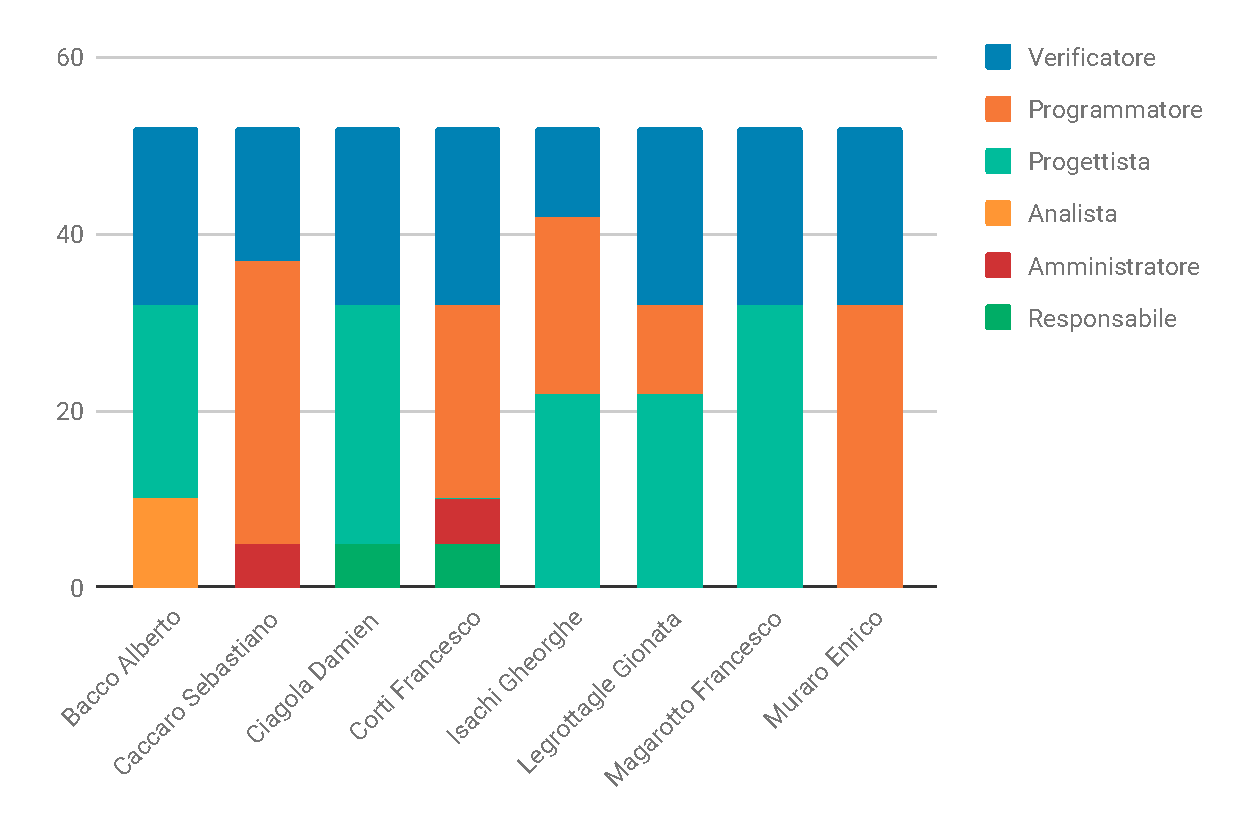
\includegraphics[width=1\linewidth]{Preventivo/grafici/PC1.pdf}
	\caption{Grafico della suddivisione oraria dei membri del gruppo nel periodo di Pianificazione di dettaglio e codifica}
\end{figure}

\subsubsection{Prospetto Economico}
Nella seguente tabella sono riportate le ore e i costi preventivati per ogni ruolo durante la fase di Pianificazione di dettaglio e codifica.


\begin{table}[H]	
	\begin{center}
	    \begin{tabular}{C{4cm}C{1cm}C{3,5cm}}
			\rowcolor{greySWEight}
			\textcolor{white}{\textbf{Ruolo}} & \textcolor{white}{\textbf{Ore}} & \textcolor{white}{\textbf{Costo in €}}
			\\ 
			Responsabile & 10 & 300,00 \\
			Amministratore & 10 & 200,00 \\
			Analista & 10 & 250,00 \\
			Progettista & 125 & 2.750,00 \\
			Programmatore & 116 & 1.740,00 \\
			Verificatore & 145 & 2.175,00 \\
			\textbf{Totale} & \textbf{416} & \textbf{7.415,00} \\
		\end{tabular}
	    \caption{Tabella della suddivisione oraria dei ruoli nel periodo di Pianificazione di dettaglio e codifica} \label{tab:tabellaRuoliPianificazione di dettaglio e codifica} 
	\end{center}
\end{table}


Si può avere una più chiara rappresentazione della distribuzione oraria dei ruoli nel seguente grafico.

\begin{figure}[H]
\centering
	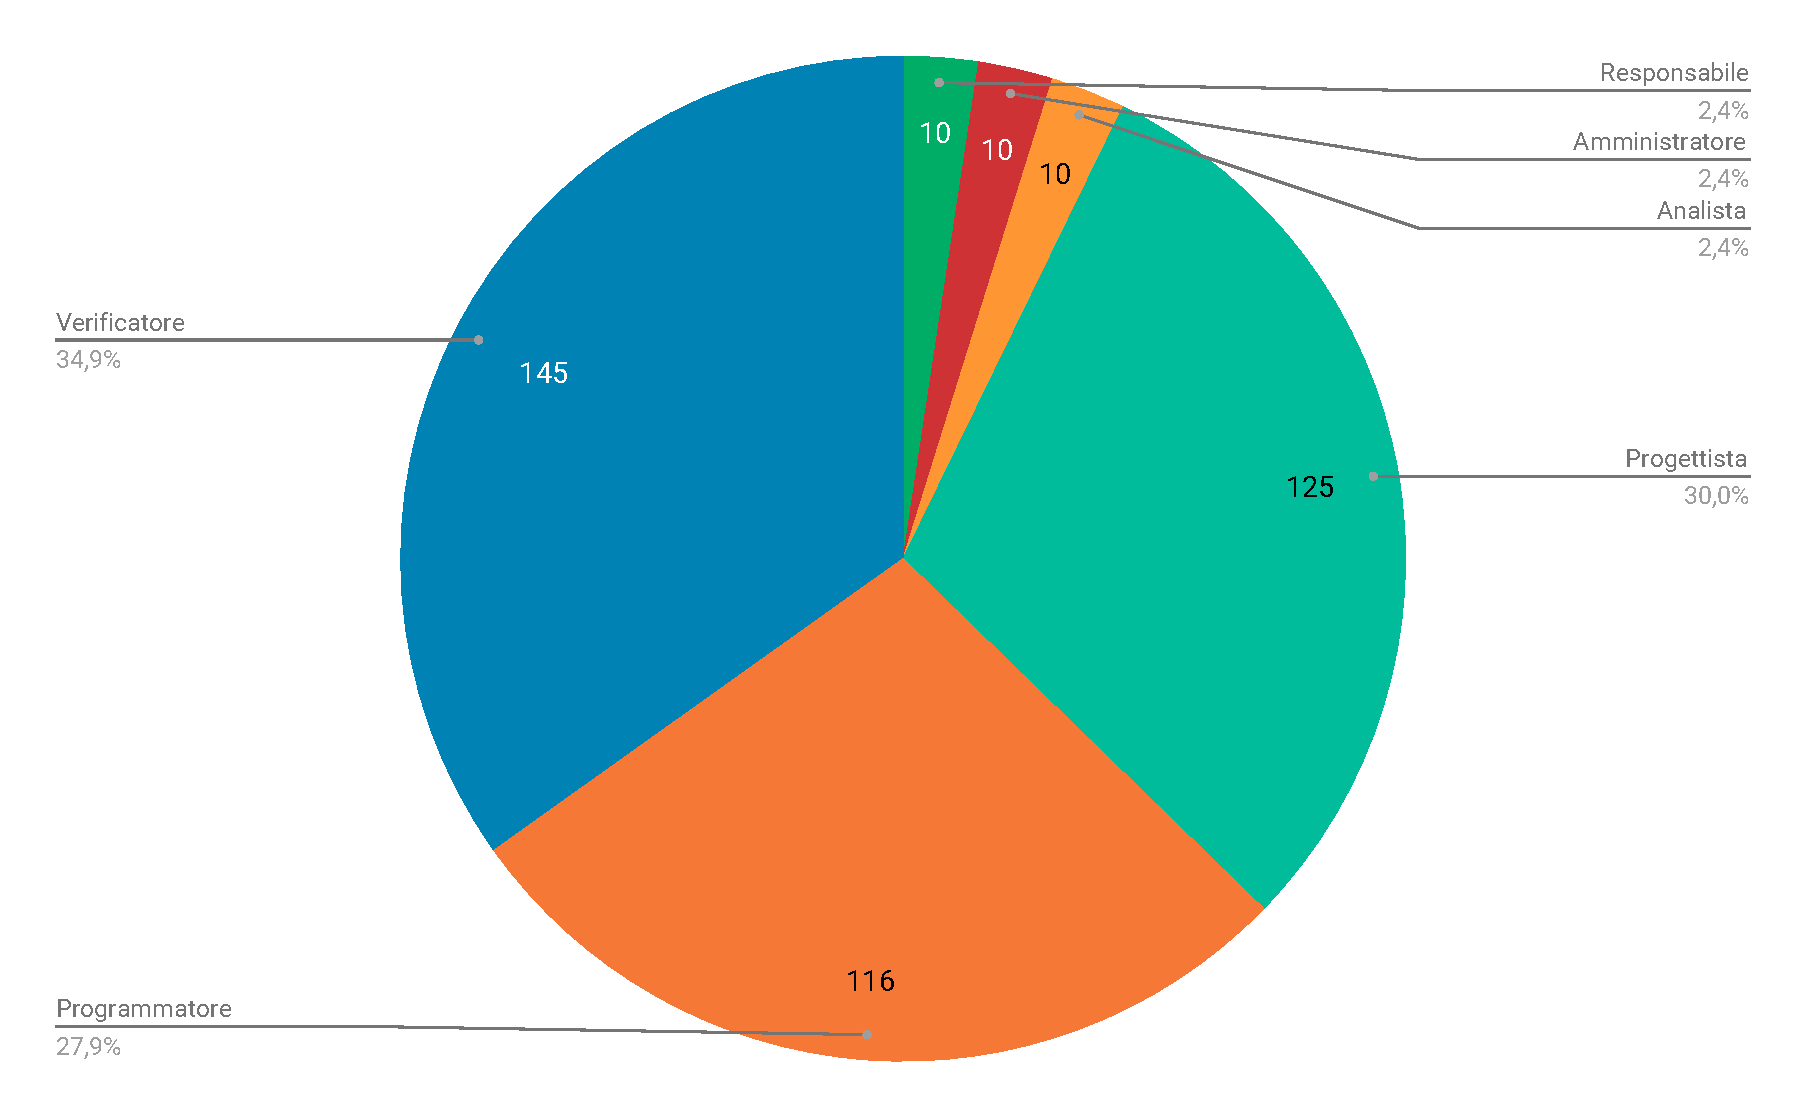
\includegraphics[width=1\linewidth]{Preventivo/grafici/PC2_1.pdf}
	\caption{Grafico della suddivisione oraria dei ruoli nel periodo di Pianificazione di dettaglio e codifica}
\end{figure}

